% WORKING DRAFT: for private review and revision, not an arXiv submission.
% Coauthors: please confirm order, affiliations, contact addresses, and contributions.
% TODO: Seek independent mathematical review of the seam-endpoint argument.
% TODO: Decide whether to include reproducible computational verification in a supplement.
% Revised copy of Wang_illumination_preprint_v01.tex. Original attachment unchanged.
% Build: pdflatex revised.tex (twice), or tectonic revised.tex.
\documentclass[11pt]{article}
\usepackage[T1]{fontenc}
\usepackage{lmodern}
\usepackage{amsmath,amssymb,amsthm,mathtools}
\usepackage{microtype}
\usepackage{geometry}
\geometry{letterpaper,margin=.9in}
\usepackage{tikz}
\usetikzlibrary{arrows.meta,calc}
\usepackage{hyperref}
\hypersetup{pdfauthor={Peyton Wang and Daniel Wang},colorlinks=true,linkcolor=black,citecolor=black,urlcolor=blue!45!black}
\usepackage{enumitem}
\setlist[itemize]{nosep,leftmargin=1.5em}
\setlength{\parindent}{0pt}
\setlength{\parskip}{3pt plus 1pt minus 1pt}
\allowdisplaybreaks
\definecolor{piecezero}{HTML}{F2E8D8}
\definecolor{pieceone}{HTML}{DCEAF2}
\definecolor{piecetwo}{HTML}{DDEDE5}
\definecolor{outline}{HTML}{233847}
\definecolor{seam}{HTML}{C78143}
\definecolor{markcolor}{HTML}{B84442}
\newtheorem{theorem}{Theorem}
\newtheorem{lemma}{Lemma}
\newtheorem{proposition}{Proposition}
\theoremstyle{remark}
\newtheorem{remark}{Remark}
\newcommand{\interior}{\operatorname{int}}
\newcommand{\corners}{\operatorname{Vert}}
\newcommand{\pathQ}{\gamma}

\title{A Simple Orthogonal 22-Gon with\\Two Non-Illuminating Interior Points}
\author{Peyton Wang\\\small Francis Parker High School \and Daniel Wang\\\small Citizen Health}
\date{Working draft v0.2 for discussion --- 2 November 2026\\\small Not submitted or peer reviewed}

\begin{document}
\maketitle
\vspace{-1.2em}
\begin{abstract}
We give exact coordinates for a strictly simple orthogonal polygon with 22 maximal sides and two distinct interior points that cannot be joined by any finite billiard trajectory avoiding polygon vertices. The room is assembled from three reflected copies of a five-square staircase. Folding a hypothetical trajectory onto the staircase reduces the problem to an elementary lattice-parity obstruction. Four smooth boundary points of the assembled room project to staircase corners; we show explicitly that reflection at these exceptional points produces only trajectory reversal and cannot evade the obstruction. The construction uses neither interior mirror partitions nor boundary self-contacts. We make no claim that 22 sides is minimal.
\end{abstract}

\section{Introduction}
In the polygonal illumination problem, light rays travel in straight lines and reflect specularly from the sides of a polygonal room. A ray that reaches a vertex is terminated. Two interior points are said to \emph{illuminate each other} if some finite trajectory with these reflection rules connects them.

Polygonal examples with non-illuminating pairs can be studied through lattice unfoldings; see \cite{Tokarsky1995,Wolecki2024}.

Our purpose is to describe an explicit \emph{strictly simple, orthogonal} 22-gon with a short elementary proof. ``Strictly simple'' means that the boundary is a Jordan polygonal curve: it has no repeated vertices, crossed edges, or self-contacts. Only the exterior boundary reflects light; the dashed segments in the construction are open passages, not mirrors. The argument is self-contained and requires no general theory of translation surfaces.

\begin{theorem}[Main result]\label{thm:main}
There exists a strictly simple orthogonal polygon $Q$ with exactly 22 maximal sides, without holes or interior mirror partitions, containing two distinct points $S,T\in\interior(Q)$ such that no finite billiard trajectory avoiding the vertices of $Q$ connects $S$ to $T$.
\end{theorem}

\section{The construction}
Let $P$ be the union of five closed unit squares with lower-left corners
\begin{equation}\label{eq:squares}
(-1,-1),\quad(0,-1),\quad(0,-2),\quad(1,-2),\quad(1,-3).
\end{equation}
Mark two smooth points of its boundary,
\begin{equation}\label{eq:ab}
a=(0,0),\qquad b=(2,-2).
\end{equation}
Take the following isometric copies of $P$:
\begin{equation}\label{eq:copies}
P_0=P,\qquad P_1=\{(x,-y):(x,y)\in P\},\qquad
P_2=\{(4-x,-y):(x,y)\in P\}.
\end{equation}
Their interiors are pairwise disjoint. The first two meet exactly along
\(H=[-1,1]\times\{0\}\), and the latter two meet exactly along
\(V=\{2\}\times[1,3]\). There are no further contacts. Set
\[
Q=P_0\cup P_1\cup P_2,\qquad S=(0,0),\quad T=(2,2).
\]
Both $S$ and $T$ are midpoints of \emph{open passages} between copies and consequently are interior points of $Q$.

\begin{figure}[htbp]
\centering
\begin{minipage}{.34\textwidth}
\centering
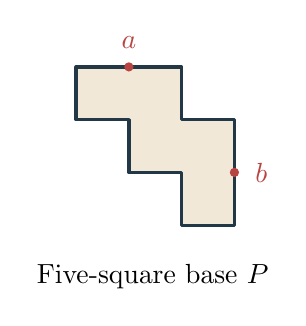
\begin{tikzpicture}[scale=.67,line cap=round,line join=round]
  \fill[piecezero] (-1,-1)--(-1,0)--(1,0)--(1,-1)--(2,-1)--(2,-3)--(1,-3)--(1,-2)--(0,-2)--(0,-1)--cycle;
  \draw[outline,very thick] (-1,-1)--(-1,0)--(1,0)--(1,-1)--(2,-1)--(2,-3)--(1,-3)--(1,-2)--(0,-2)--(0,-1)--cycle;
  \fill[markcolor] (0,0) circle (2.5pt) node[above=3pt] {$a$};
  \fill[markcolor] (2,-2) circle (2.5pt) node[right=4pt] {$b$};
  \node[align=center,below] at (.45,-3.55) {Five-square base $P$};
\end{tikzpicture}
\end{minipage}\hfill
\begin{minipage}{.62\textwidth}
\centering
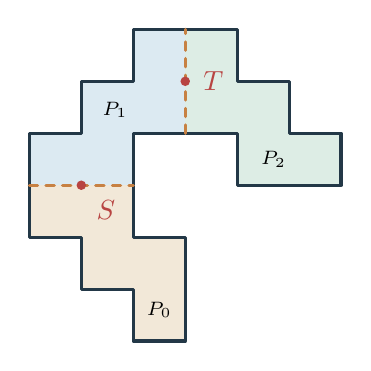
\begin{tikzpicture}[scale=.66,line cap=round,line join=round]
  \fill[piecezero] (-1,-1)--(-1,0)--(1,0)--(1,-1)--(2,-1)--(2,-3)--(1,-3)--(1,-2)--(0,-2)--(0,-1)--cycle;
  \fill[pieceone] (-1,1)--(-1,0)--(1,0)--(1,1)--(2,1)--(2,3)--(1,3)--(1,2)--(0,2)--(0,1)--cycle;
  \fill[piecetwo] (2,3)--(3,3)--(3,2)--(4,2)--(4,1)--(5,1)--(5,0)--(3,0)--(3,1)--(2,1)--cycle;
  \draw[outline,very thick] (-1,-1)--(0,-1)--(0,-2)--(1,-2)--(1,-3)--(2,-3)--(2,-1)--(1,-1)--(1,1)--(3,1)--(3,0)--(5,0)--(5,1)--(4,1)--(4,2)--(3,2)--(3,3)--(1,3)--(1,2)--(0,2)--(0,1)--(-1,1)--cycle;
  \draw[seam,dashed,line width=1.15pt] (-1,0)--(1,0) (2,1)--(2,3);
  \fill[markcolor] (0,0) circle (2.6pt) node[below right=2pt] {$S$};
  \fill[markcolor] (2,2) circle (2.6pt) node[right=3pt] {$T$};
  \node at (1.5,-2.4) {\scriptsize $P_0$};
  \node at (.65,1.45) {\scriptsize $P_1$};
  \node at (3.7,.5) {\scriptsize $P_2$};
\end{tikzpicture}
\end{minipage}
\caption{The five-square base $P$ and the 22-sided room $Q$. The bold exterior outline is reflective. The dashed segments are open seams, not partitions. The two marked points $S$ and $T$ lie in the interior of $Q$.}\label{fig:construction}
\end{figure}

For reproducibility, the counterclockwise sequence of all 22 vertices of $Q$ is
\begin{equation}\label{eq:vertices}
\begin{gathered}
(-1,-1), (0,-1), (0,-2), (1,-2), (1,-3), (2,-3),\\
(2,-1), (1,-1), (1,1), (3,1), (3,0), (5,0),\\
(5,1), (4,1), (4,2), (3,2), (3,3), (1,3),\\
(1,2), (0,2), (0,1), (-1,1).
\end{gathered}
\end{equation}
Every successive edge is horizontal or vertical and nonzero, with successive edges meeting at right angles. The union description (or a direct check of the vertex cycle) shows that the boundary does not self-intersect or self-touch. There are 13 convex vertices and nine reflex vertices, and the area is 15.

The \emph{folding map} $f:Q\to P$ is defined copywise by
\begin{equation}\label{eq:fold}
f|_{P_0}(x,y)=(x,y),\qquad
f|_{P_1}(x,y)=(x,-y),\qquad
f|_{P_2}(x,y)=(4-x,-y).
\end{equation}
These formulas agree on the seams, so $f$ is well defined and continuous. In particular, $f(S)=a$ and $f(T)=b$.

\section{The lattice obstruction on the staircase}
The next lemma concerns \emph{ordinary} billiard motion in $P$, reflecting only at smooth boundary points and never touching a vertex. Paths have finitely many nonzero straight legs. At each intermediate smooth-wall contact the incoming and outgoing legs satisfy the specular reflection rule.

\begin{lemma}[Parity obstruction]\label{lem:parity}
There is no finite corner-avoiding billiard path in $P$ from $a=(0,0)$ to $b=(2,-2)$.
\end{lemma}
\begin{proof}
First inspect the integer points in $P$. There are no interior integer points. Its only integer boundary points that are not vertices are $a$ and $b$. More explicitly, its seven convex corners are
\[
(-1,-1),\ (-1,0),\ (0,-2),\ (1,-3),\ (1,0),\ (2,-3),\ (2,-1),
\]
and its three reflex corners are
\[
(0,-1),\ (1,-2),\ (1,-1).
\]

Suppose an ordinary billiard path from $a$ to $b$ exists. Unfold its finitely many reflections, reflecting the staircase instead of bending the path. The result is a single straight segment starting at $a=(0,0)$ and ending at an image $B$ of $b$. Reflection across any wall $x=c$ or $y=d$, where $c,d\in\mathbb{Z}$, preserves both coordinate parities. Since $b$ has even coordinates, $B\in(2\mathbb{Z})^2$. Further, $B\ne(0,0)$ because unfolding preserves the positive length of the path.

Write $B=2^r z$, where $r\ge 1$ and $z\in\mathbb{Z}^2$ has at least one odd coordinate; choose $r$ maximal. Then $z$ is a lattice point strictly between $0$ and $B$ on the unfolded segment. Fold $z$ back to $P$ along the proposed itinerary. All inverse unfolding maps are compositions of reflections in integer-coordinate lines and therefore preserve integrality and coordinate parities. The image of $z$ is an integer point of $P$ with an odd coordinate. It is neither $a$ nor $b$, hence must be a vertex of $P$. This would make the original path hit a vertex, a contradiction.
\end{proof}

\begin{remark}
The lemma is valid for arbitrary finite path length, direction, and number of reflections. The obstruction arises from the parity of an \emph{unfolded endpoint}, not from a bounded search over directions.
\end{remark}

\section{What happens at the seams?}
A billiard trajectory in $Q$ need not fold into an ordinary billiard trajectory in $P$ at every instant. The exceptions are precisely the smooth boundary points of $Q$ lying at the ends of open seams. It is important to account for them rather than treating them as forbidden corners of $Q$.

Away from the seams, each branch of $f$ is an isometry. A reflection at a smooth exterior wall of $Q$ thus becomes an ordinary reflection at a smooth wall of $P$, unless that point is a seam endpoint. A straight passage across the \emph{interior} of either seam also becomes an ordinary reflection in $P$: the adjacent folding maps agree at the seam and reverse the normal component of velocity.

The four seam endpoints are
\begin{equation}\label{eq:exceptional}
E_1=(-1,0),\qquad E_2=(1,0),\qquad
E_3=(2,1),\qquad E_4=(2,3).
\end{equation}
Each $E_j$ is smooth on the external boundary of $Q$, yet folds to a convex right-angle corner of $P$:
\[
\begin{array}{c|c|c}
\text{smooth point of }Q & \text{vertex of }P & \text{exterior mirror in }Q\\ \hline
(-1,0) & (-1,0) & \text{vertical}\\
(1,0) & (1,0) & \text{vertical}\\
(2,1) & (2,-1) & \text{horizontal}\\
(2,3) & (2,-3) & \text{horizontal}
\end{array}
\]

\begin{lemma}[Seam-endpoint reversal]\label{lem:reversal}
If a corner-avoiding billiard trajectory in $Q$ reflects at a seam endpoint $E_j$, its folded trajectory in $P$ instantaneously \emph{reverses its entire velocity} at the corresponding convex corner and retraces its incoming route.
\end{lemma}
\begin{proof}
For example, consider $E_2=(1,0)$. A ray approaching from $P_1$ with physical velocity $(u,-v)$ ($u,v>0$) folds via $(x,y)\mapsto(x,-y)$ to incoming velocity $(u,v)$ in $P$. At $E_2$, the actual exterior mirror is vertical, so the physical outgoing velocity becomes $(-u,-v)$ and the ray travels into $P_0$. Folding this outgoing segment by the identity gives $(-u,-v)$, the negative of the incoming folded velocity. Reversing the time orientation gives the same conclusion for arrivals from $P_0$.

At $E_1$ the same two reflections occur in the opposite horizontal direction. At $E_3$ and $E_4$, interchange the horizontal and vertical coordinates: the physical exterior reflection negates the vertical component, while switching copies across the vertical seam negates the horizontal component. In every case, the combined effect is $(p,q)\mapsto(-p,-q)$.
\end{proof}

\begin{figure}[htbp]
\centering
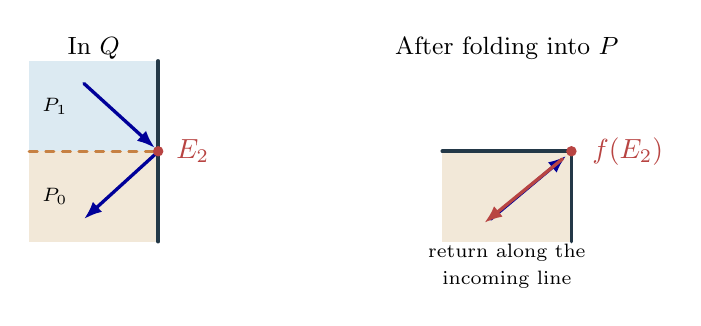
\begin{tikzpicture}[>=Latex,scale=.82,line cap=round]
  \begin{scope}
    \fill[pieceone] (-1,0) rectangle (1,1.4);
    \fill[piecezero] (-1,-1.4) rectangle (1,0);
    \draw[outline,line width=1.3pt] (1,-1.4)--(1,1.4);
    \draw[seam,dashed,line width=1pt] (-1,0)--(1,0);
    \draw[blue!60!black,very thick,-{Latex[length=2.3mm]}] (-.15,1.05)--(.95,.05);
    \draw[blue!60!black,very thick,-{Latex[length=2.3mm]}] (.95,-.05)--(-.15,-1.05);
    \fill[markcolor] (1,0) circle(2.3pt) node[right=3pt] {$E_2$};
    \node at (0,1.6) {\small In $Q$};
    \node at (-.6,.7) {\scriptsize $P_1$};
    \node at (-.6,-.7) {\scriptsize $P_0$};
  \end{scope}
  \begin{scope}[xshift=6.4cm]
    \fill[piecezero] (-1,-1.4) rectangle (1,0);
    \draw[outline,line width=1.3pt] (-1,0)--(1,0)--(1,-1.4);
    \draw[blue!60!black,very thick,-{Latex[length=2.3mm]}] (-.25,-1.05)--(.92,-.07);
    \draw[markcolor,very thick,-{Latex[length=2.3mm]}] (.86,-.12)--(-.35,-1.11);
    \fill[markcolor] (1,0) circle(2.3pt) node[right=4pt] {$f(E_2)$};
    \node at (0,1.6) {\small After folding into $P$};
    \node[align=center] at (0,-1.78) {\scriptsize return along the\\[-2pt]\scriptsize incoming line};
  \end{scope}
\end{tikzpicture}
\caption{The exceptional event at the horizontal seam endpoint $E_2$. A normal mirror reflection in $Q$ switches copies and becomes an exact retracing at a convex vertex of $P$. The diagrams show local geometry, not a possible complete connecting path.}\label{fig:reverse}
\end{figure}

Every original corner of $P$ gives one corner incidence in each of $P_0,P_1,P_2$. Of these 30 incidences, two meet at each of the four smooth endpoints $E_j$ (eight incidences total). All remaining 22 incidences are actual vertices of $Q$. In particular, \emph{no reflex corner of $P$ is the image of a smooth point of $Q$}. It follows that a valid $Q$-trajectory can fold only to ordinary billiard motion in $P$, occasionally interrupted by the corner reversals of Lemma~\ref{lem:reversal}.

\section{Why reversals do not create a connecting path}
\begin{lemma}[Reversals do not help]\label{lem:nohelp}
There is no finite path from $a$ to $b$ in $P$ obtained by ordinary billiard reflections at smooth walls together with the additional rule that a path may reverse its velocity and retrace itself at a convex corner. Reflex corners remain forbidden.
\end{lemma}
\begin{proof}
Suppose such a path exists. Stop it at its first arrival at $b$, and retain only the subpath beginning at its \emph{last} visit to $a$ before that arrival. The resulting path $\gamma$ starts at $a$, ends at $b$, and contains no interior occurrence of either marked point. There are finitely many such visits because the path has finitely many nonzero straight legs. This truncation takes place in $P$: a visit to $a$ counts regardless of which preimage of $a$ the original path visits in $Q$.

Assume $\gamma$ has a corner reversal, and choose the first one. Up to that event, motion consists entirely of ordinary billiard reflections. Ordinary billiard motion is deterministic and reversible. Once the first reversal takes place, the path must retrace the entire preceding route in reverse order, ultimately reaching $a$. It cannot reach $b$ during this retracing, since the corresponding point would already have occurred before the reversal, contradicting the first-arrival choice of $b$. Thus the path revisits $a$ before reaching $b$, contradicting the last-visit choice of $a$.

Hence $\gamma$ has no reversals and is an ordinary corner-avoiding billiard path from $a$ to $b$, contrary to Lemma~\ref{lem:parity}.
\end{proof}

\begin{proof}[Proof of Theorem~\ref{thm:main}]
The explicit construction and boundary cycle establish that $Q$ is a strictly simple orthogonal polygon with 22 maximal sides, no holes, and $S,T\in\interior(Q)$.

Suppose a finite billiard trajectory joins $S$ to $T$ in $Q$. It cannot be axis-parallel: reflecting in a horizontal or vertical wall preserves the property that one velocity component vanishes, whereas $S$ and $T$ differ in both coordinates. Consequently every straight leg meets either seam transversely, if at all. Since the trajectory has finitely many legs and each leg crosses each seam at most once, its folding by $f$ splits into finitely many straight segments and events.

By the seam analysis, the image is a finite path from $a=f(S)$ to $b=f(T)$ following the rules of Lemma~\ref{lem:nohelp}. That lemma forbids such a path. Therefore no finite corner-avoiding billiard trajectory joins $S$ and $T$.
\end{proof}

\section{Discussion and scope}
This example uses a connected, simply connected, axis-aligned room whose 22 boundary edges are all genuine exterior mirrors. The two marked points are interior points, rather than points of the reflective boundary. The proof's key components are a mod-2 obstruction after unfolding and an explicit treatment of the four points where a smooth wall of the assembled room maps to a corner of the base staircase.

The proof is independent of the computational searches that helped identify the example. The reversal principle is consistent with the usual continuation through removable corners; see \cite[Remark~2.2]{Wolecki2024}.

\paragraph{Acknowledgements and AI assistance.}
The authors used the AI systems ChatGPT (OpenAI) and Claude (Anthropic) extensively while exploring candidate geometries, developing explanations, and refining the proof. The authors take responsibility for the mathematical content of any eventual submitted version.

\begin{thebibliography}{9}
\bibitem{Tokarsky1995}
G.~W. Tokarsky, ``Polygonal Rooms Not Illuminable from Every Point,''
\emph{The American Mathematical Monthly} \textbf{102} (1995), no.~10, 867--879.
\url{https://doi.org/10.1080/00029890.1995.12004679}.

\bibitem{Wolecki2024}
A.~Wolecki, ``Illumination in Rational Billiards,''
\emph{arXiv:1905.09358v3} (2024), Theorem~1.3, Figure~1, and Acknowledgements.
\url{https://arxiv.org/abs/1905.09358v3}.
\end{thebibliography}
\end{document}
